\section{Parametrization of the functions}

As we said above, the functions $f$ and $g$ must be parametrized.
The authors propose the following for $f$ and $g$ :

\begin{align*}
  f(x,u) &= \sum_{i=1}^I \rho_i(x) h_i + Ax + Bu + b\\
  g(x,u) &= \sum_{j=1}^J \rho'_j(x) k_j + Cx + Du + d\\ \\
   % nice functions output
    \rho_i(x) &\colon
	\begin{array}{ccl}
   		\mathbb{R}^p &\to & \mathbb{R}\\
   		x &\mapsto & \dfrac{1}{(2\pi)^{d/2}|S_i|^{1/2}} \exp\left(-			\dfrac{1}{2}(x-c_i)^T S_{i}^{-1}(x-c_i)\right)\\
	\end{array}\\ \\
  \rho'_j(x) & \colon
	\begin{array}{ccl}
		\mathbb{R}^p &\to & \mathbb{R}\\
	 	x &\mapsto & \dfrac{1}{(2\pi)^{d/2}|S'_j|^{1/2}} \exp\left(-		\dfrac{1}{2}(x-c'_j)^T {S'_{j}}^{-1}(x-c'_j)\right)\\
	\end{array} \\ \\
A \in \mathbb{R}^{p \times p}, & \  B \in \mathbb{R}^{p \times q}, \  C \in \mathbb{R}^{n \times p}, \  D \in \mathbb{R}^{n \times q}\\
  h_i \in \mathbb{R}^{p},& \  b \in \mathbb{R}^p, \  k_j \in \mathbb{R}^{n},\   d \in \mathbb{R}^n\\
\end{align*}

The real valued functions $\rho_i$ and $\rho'_j$ are called radial basis functions (RBF). The \textit{radial} terminology represent the dependency on the hilbertian distance (induced by the p.s.d matrix $S_i$) to a center $c_i$.
\textbf{The centers $c_i$ and $c'_j$ of the RBF are supposed to be known, as well as the width $S_i$ and $S'_j$}. Actually they are a sort of hyper-parameters for this method and we'll discuss later of a good way to set them but, for the moment, we suppose them as fixed since they will not be learned in the EM.


To sum things up, $f$ is the sum of an affine function ($x \rightarrow Ax + b$) with a linear combination of $I$ radial basis functions ($x \mapsto \rho_i(x)$, $i=1 \cdots I$).
The parameters $\theta_f$ and $\theta_g$ of our functions are :
\begin{eqnarray*}
  \theta_f &= \left( h_1, \ldots , h_I, A, B, b\right)  \in \mathbb{R}^{p \times (I+p+q+1)}\\
  \theta_g &= \left( k_1, \ldots , k_J, C, D, d\right) \in \mathbb{R}^{n \times (J+p+q+1)}
\end{eqnarray*}
The following plots present examples of such functions, when we use no inputs $u$ and set the state dimension to 1 ($p = 1$)\. The functions $f_I : \mathbb{R} \to \mathbb{R}$ where plotted on the segment $\left [ 0 , 1 \right ]$:

\begin{figure}[H]
\captionsetup{labelformat=empty}
\minipage{0.32\textwidth}
  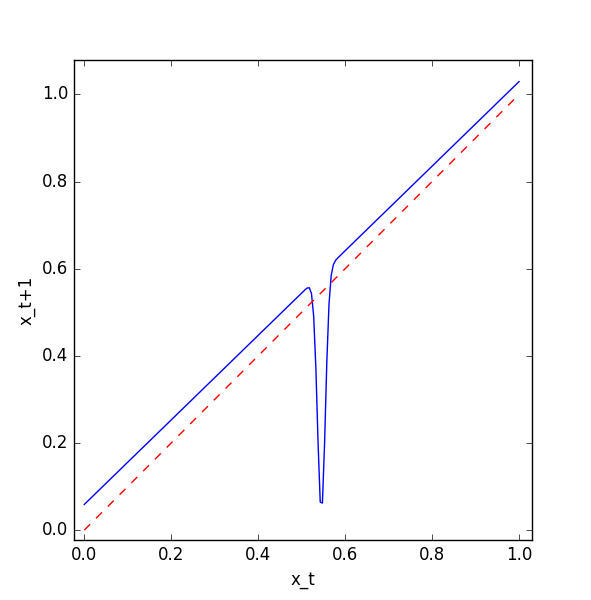
\includegraphics[width=\linewidth]{function_RBF_3.png}
  \caption{I = 1}
\endminipage\hfill
\minipage{0.32\textwidth}
  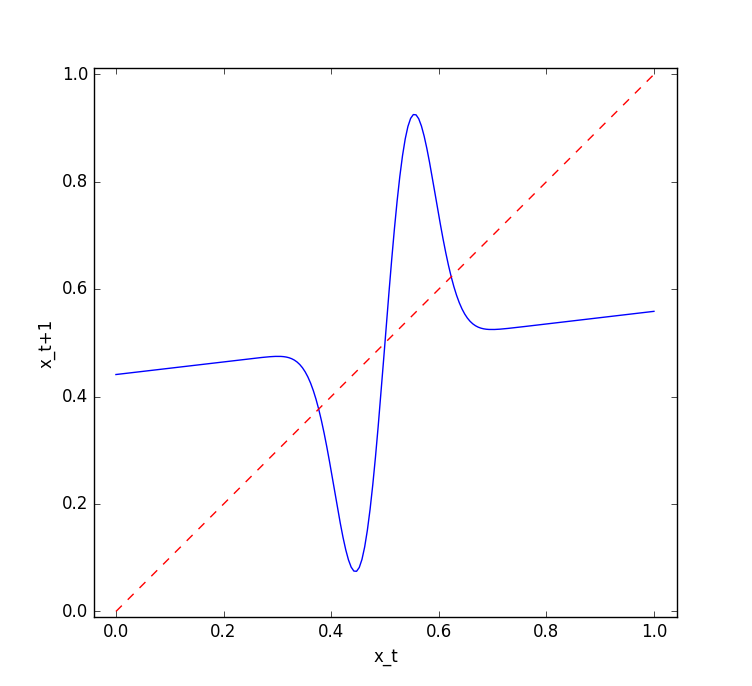
\includegraphics[width=\linewidth]{function_RBF_1.png}
  \caption{I = 2}
\endminipage\hfill
\minipage{0.32\textwidth}
  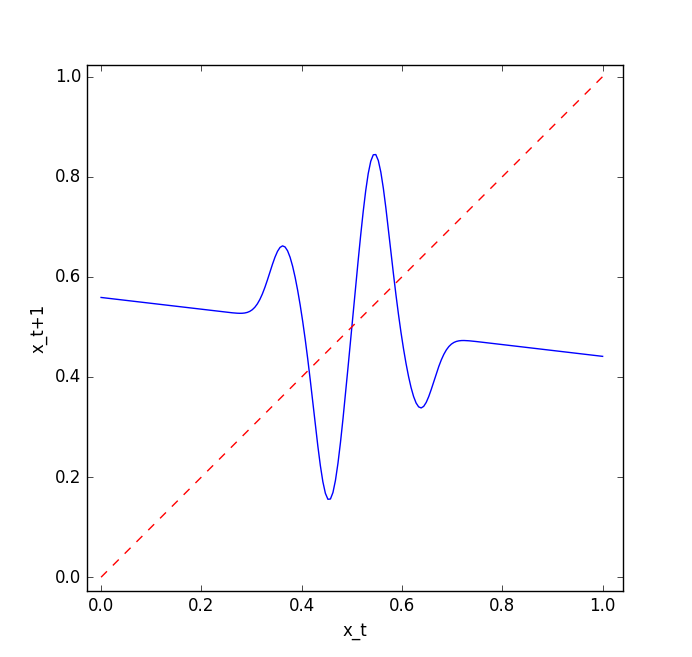
\includegraphics[width=\linewidth]{function_RBF_2.png}
  \caption{I = 4}
\endminipage\hfill
\end{figure}

Now that the functions $f$ and $g$ are parametrized, we can begin with the study of the proposed EM algorithm.
